\RequirePackage[l2tabu, orthodox]{nag}
\documentclass[a4paper]{article}
\usepackage[utf8]{inputenc}
\usepackage[T1]{fontenc}
\usepackage{lmodern}
\usepackage[pdftex, hidelinks,
            pdftitle={Flödesanimering i Realtid med 3-D Curlbrus},
            pdfauthor={Martin Estgren and and Rasmus Hedin and Alfred Rundquist and Erik S. V. Jansson},
            pdfsubject={Computer Graphics -- Animation -- Physical Simulation / Procedural Animation},
            pdfkeywords={curl-noise,animation,fluid simulation,navier-stokes,gpu,real-time}]{hyperref}

\usepackage{bm}
\usepackage{caption}
\usepackage{listings}
\usepackage{mathtools}
\usepackage[margin=0.8in]{geometry}
\usepackage[parfill]{parskip}
\usepackage[swedish]{babel}
\usepackage{algorithmic}
\usepackage{graphicx}
\usepackage{courier}
\usepackage{hyperref}
\usepackage{amsmath}
\usepackage{amssymb}
\usepackage{algorithm}
\usepackage{multicol}
\setlength{\columnsep}{0.5cm}
\usepackage[capitalize, noabbrev]{cleveref}
\usepackage[activate={true, nocompatibility}, final,
            tracking=true, kerning=true, spacing=true,
            factor=1100, stretch=10, shrink=10]{microtype}

\DeclareCaptionFormat{modifiedlst}{\rule{\textwidth}{0.85pt}\\[-2.9pt]#1#2#3}
\captionsetup[lstlisting]{format =  modifiedlst,
labelfont=bf,singlelinecheck=off,labelsep=space}
\lstset{basicstyle=\footnotesize\ttfamily,
        breakatwhitespace = false,
        breaklines = true,
        keepspaces = true,
        language = C++,
        showspaces = false,
        showstringspaces = false,
        frame = tb,
        numbers = left,
        numbersep = 5pt,
        xleftmargin = 16pt,
        framexleftmargin = 16pt,
        belowskip = \bigskipamount,
        aboveskip = \bigskipamount,
        escapeinside={<@}{@>}}

\date{\vspace{-0.5ex}} % Buys us some space.
\title{\vspace{-2.2cm}\textbf{Flödesanimering i Realtid med 3-D Curlbrus}\\
       \Large{\textit{--- en kort teknisk saga angående dess fasor och dess under ---}}\vspace{-0.25cm}}
\author{{\textbf{Martin Estgren}}\;\;\;\;\;\; {\href{mailto:mares480@student.liu.se}{\texttt{<mares480@student.liu.se>}}}\\
        {\textbf{Rasmus Hedin}}\;\;\;\;\;\;\;\; {\href{mailto:rashe877@student.liu.se}{\texttt{<rashe877@student.liu.se>}}}\\
        {\textbf{Alfred Rundquist}}\;\;\; {\href{mailto:alfru536@student.liu.se}{\texttt{<alfru536@student.liu.se>}}}\\
        {\textbf{Erik S. V. Jansson}}\; {\href{mailto:erija578@student.liu.se}{\texttt{<erija578@student.liu.se>}}}}

\begin{document}
    \maketitle
\begin{multicols}{2}

    \section{Introduktion}

    Ett viktigt område inom \emph{datorgrafik och visualisering} är förmågan att \emph{simulera}/\emph{animera} verklighetstrogna \emph{flödessystem} i \emph{realtid}. Dessa används i bl.a. spel och filmer för att enkelt skapa \emph{visuella effekter} som t.ex. \emph{rök- och vattenrörelser}; effekter som vanligtvis inte görs ``för hand'', och är mer lämpliga att genereras av en dator. I detta projekt så har vi implementerat ett \emph{grundläggande flödessystem} för att \emph{animera ett partikelsystem} i 3-D med hjälp av den så kallade \emph{Curl-Noise} (``curlbrus''), först presenterad av \emph{Bridson et al.}~\cite{bridson2007curl} i 2007.

    \textit{Curlbrus} används för att framställa verklighetstrogna \emph{partikelflöden} genom att \emph{procedurellt animera turbulenta flöden}. Detta görs genom att skapa \emph{procedurellt brus}, som används för att skapa ett \emph{divergens-fritt vektorfält} genom att applicera billiga vektorfältsoperationer. Detta är en billigare variant av \emph{Navier-Stokes}, som är fysiskt korrekt; men eftersom vi endast är efter dess visuella egenskaper, så är Curlbrus tillräckligt bra. Dessutom så kan Curlbrus beräknas i realtid, vilket gör den lämplig för integrering i t.ex. spel och infovis.

    Målet med detta projekt var att skapa ett enkelt \emph{3-D partikelsystem} där rörelsen bestäms av ett riktningsfält genererat genom \emph{Curlbrus metoden}. Dessutom så producerades det några enkla \emph{visuella effekter}.

    Den preliminära arbetsprocessen gick ut på att vi parprogrammerade med versionshantering via \textit{Git}. För att realisera partikelsystemet valde vi att använda \textit{OpenCL} för partikelberäkningar, \textit{OpenGL} för rendering, \textit{GLFW} för fönsterhantering, \textit{AntTweakbar} för ``run-time'' konfigurering, och \textit{GLEW} för att hantera \textit{OpenGL}-tillägg. Själva koden skrevs i C++, där våra kernels skrevs i \textit{OpenCLs} variant av C, samt shaders i \textit{GLSL}.

    \vspace{-0.4cm}
    \section{Teori och metodik}
    \subsection{Systemöversikt}

    Vid tidpunkten \(t_n\) så befinner sig varje partikel vid sin egen position \(\vec{x}\), lagrade i en \emph{buffer}. Målet är att räkna ut partikelns nästa position \(\vec{x}'\) vid tidpunkten \(t_{n+1}\) (d.v.s. vi stegar fram simuleringen). Detta görs genom \(\vec{x}' = \vec{x} + \mathbf{V}(\vec{x})\), där \(\mathbf{V}(\vec{x})\) är \emph{fältriktningen}. Allt detta hanteras av \emph{partikelsystemet}, där dessutom \(\mathbf{V}(\vec{x})\) skapas, och beskrivs väl under Rubrik~\ref{sec:partikelsystemet}. Detta görs parallelt på \emph{grafikprocessorn} (GPU) för varje partikel under samma \(t_n\). Vilket gör att positionerna \(\vec{x}'\) kan återanvändas när vi skall \emph{visualisera} dem med våran \emph{partikelrenderare}, då båda systemen behöver ej lämna grafikprocessorns minnesrymd. Se Figur~\ref{fig:system}.

    \begin{figure}[H]
    \center
    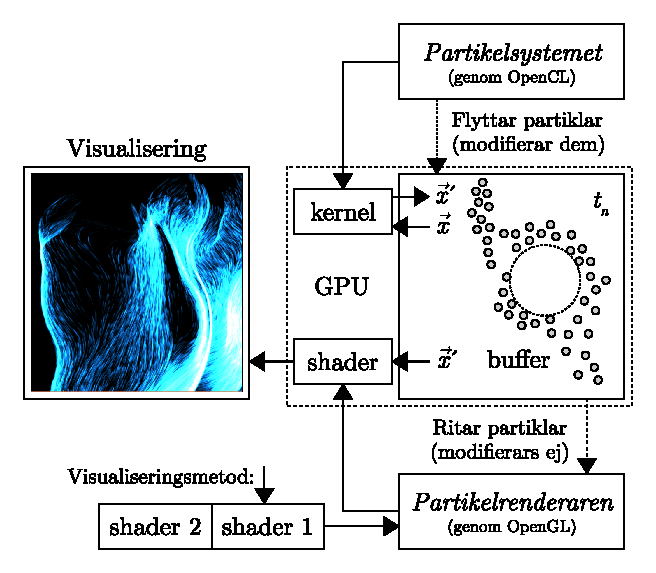
\includegraphics[width=0.5\textwidth]{share/System.eps}
    \caption{konceptuell översikt över våra två subsystem.}
    \label{fig:system}
    \end{figure}

    Detta görs genom att ladda upp en \emph{kernel} (beräkningskärna) som läser in \(\vec{x}\) och därefter skriver över denna med \(\vec{x}'\). Genom att läsa \(\vec{x}'\) från den delade buffern så kan en \emph{shader} användas för att rita partiklarna, genom att tolka hela \(\vec{x}'\) som en \emph{vertex buffer}. Man kan enkelt ändra \emph{visualiseringsmetod} (hur man ritar \(\vec{x}'\)) genom att byta shader, vilket beskrivs under Rubrik~\ref{sec:partikelrenderaren}.

    \vspace{-0.35cm}
    \subsection{Partikelsystemet} \label{sec:partikelsystemet}

    Varje partikel beräknas parallellt i Grafikprocessorn genom \textit{OpenCL} där följande operationer utförs för varje partikels koordinater.

    I originalpapperet presenteras både beräkningarna för två och tre dimensioner men eftersom vi valt att enbart implementera den sistnämnda fokuserar vi på den. Vi kommer ej heller följa originalpapperets beräkningar exakt utan justerar så det passar vårat system bättre. Vidare har några förändringar gjorts för att bättre anpassa vektorfältet till vårat system.

    I korthet kan man säga att vi producerar tre olika vektorfält som vi kombinerar. De första två fälten representerar turbulensen och den allmänna riktningen som partiklarna ska följa som vi kombinerar genom att addera de resulterande fälten. Efter detta modifierar vi fältet så att den leder partiklar runt solida kroppar och slutligen applicerar vi en rotationsoperation (curl) vilket leder till ett divergensfritt vektorfält.

    \textbf{Turbulensen}

    Turbulensen beräknas genom att sampla en brusfunktion. Vi valde att använda \textit{Simplex noise}\footnote{\url{https://github.com/stegu/perlin-noise/blob/master/src/simplexnoise1234.c}} vilket förklaras av S. Gustavsson\cite{gustavson2005simplex} för procentuellt brus varpå vi samplar runt varje partikels position enligt följande funktion.
    \begin{equation}
   \vec{N}(\vec{x}) =  
        \begin{pmatrix}
        n((\vec{x} + \vec{\epsilon}_x)/L)
        \\
        n((\vec{x} + \vec{\epsilon}_y)/L)
        \\ 
        n((\vec{x} + \vec{\epsilon}_z)/L)
        \end{pmatrix} * \gamma M_nL
    \end{equation}
    Där $\vec{\epsilon}$ representerar en förskjutning så att inte alla komponenter får exakt samma värde, i detta fall $\vec{\epsilon} = \begin{pmatrix}
8 & 0 & 0\\ 
0 & 8 & 0\\ 
0 & 0 & 8
\end{pmatrix}$. $n(\vec{x})$ är brusfunktionen som samplas för att producera turbulens i fältet. $\gamma$ representerar förhållande mellan brus och bakgrundsfält där $0$ är inget brus och därmed ingen turbulens medan $1$ är fullt brus utan något bakgrundsfält. $M_n$ är styrkan på bruset (fältriktningen är normerad så vi skalar upp det till vad vi vill ha). $L$ är längdskalan på bruset vilket i vårat fall är relativt stor (20-100) då vi vill ha långa övergångar i bruset.
\begin{figure}[H]
\center
\begin{minipage}[]{0.3\textwidth}

\includegraphics[width=\textwidth]{share/Noise_downscale.png}
\caption{Genomskärning av turbulensfältet.}
\end{minipage}
\end{figure}

\textbf{Bakgrundsriktningen}

Bakgrundsriktningen representerar den generella riktningen vi vill att partiklarna ska följa. Detta beskrivs inte något vidare i referensartikeln. Vi valde istället att anpassa en redan existerande implementation\footnote{\url{https://github.com/kbladin/Curl_Noise/blob/master/shaders/point_cloud_programs/update_velocities_curl_noise.frag}} av K. Bladin, vilket resulterar i ett relativt enkelt bakgrundsfält som går i en uniform riktning.
\begin{equation}
     \vec{F}(\vec{x}) = (1.0-\gamma) *  \vec{D}(\vec{x}) * M_f
\end{equation}
$ \vec{D}(\vec{x})$ representerar fältriktningen i den angivna punkten. Fältriktningen är beräknad enligt följande formel
\begin{equation}
    \vec{D}(\vec{x}) = \vec{x} \times \vec{p}
\end{equation}
Där $\vec{p}$ är fältriktningen vi har valt att partiklarna ska följa.

\begin{figure}[H]
\center
\begin{minipage}[]{0.3\textwidth}

\includegraphics[width=\textwidth]{share/Background_downscale.png}
\caption{Genomskärning av bakgrundsfället.}
\end{minipage}
\end{figure}

Brusriktningen adderas med bakgrundsriktningen ($\vec{\psi} = \vec{N}(\vec{x}) + \vec{F}(\vec{x})$) för att sedan justeras så att partiklarna beaktar solida sfärer utplacerade i vektorfältet. 

\textbf{Solida kroppar i fältet}

För att få alla partiklar att respektera de sfärer vi placerat i fältet använder vi rampfunktionen
\begin{equation}
ramp(r) = \left\{\begin{matrix}
1  && r > 1
\\
6r^4 - 15r^4 + 10r^3 && 0 \le r \le 1
\\ 
0  && r < 0
\end{matrix}\right.
\end{equation}
där $r$ är skillnaden mellan distansen $\vec{x}$ och den närmsta sfären delat på marginalen runt sfären. 
\begin{figure}[H]
\center
\begin{minipage}[]{0.3\textwidth}

\includegraphics[width=\textwidth]{share/Alpha_downscale.png}
\caption{Genomskärning av ramp funktionen mot en sfärisk solid kropp.}
\end{minipage}
\end{figure}

För att få partiklarna att gå runt sfärerna använder vi nu resultatet från rampfunktionen som $\alpha = | ramp(d(\vec{x})/d_0) |$ där $d_0$  är en arbiträr skalfaktor. Slutligen beräknar vi hur fältet runt sfären ska se ut genom 
\begin{equation}
\vec{\psi}_c(\vec{x}) = \alpha * \vec{\psi}(\vec{x}) + (1.0 - \alpha) * \vec{x} * \vec{\psi}(\vec{x}) \cdot \vec{x}
\end{equation}
vilket producerar en övergång från fältriktningen till en riktning tangentiell mot sfären.

\textbf{Curl}

Vi får fram $ \nabla \vec{\psi}$ genom en \textit{finit differensmetod}
\begin{equation}
\vec{vx} = \vec{\psi}_c(\vec{x} + \vec{\epsilon}_x  ) - \vec{\psi}_c(\vec{x} - \vec{\epsilon}_x  )
\end{equation}
\begin{equation}
\vec{vy} = \vec{\psi}_c(\vec{x} + \vec{\epsilon}_y  ) - \vec{\psi}_c(\vec{x} - \vec{\epsilon}_y  )
\end{equation}
\begin{equation}
\vec{vz} = \vec{\psi}_c(\vec{x} + \vec{\epsilon}_z  ) - \vec{\psi}_c(\vec{x} - \vec{\epsilon}_z  )
\end{equation}
där $\vec{\epsilon} = \begin{pmatrix}
0.0001 & 0 & 0\\ 
0 & 0.0001 & 0\\ 
0 & 0 & 0.0001
\end{pmatrix}$ och varje resultatvektor $\vec{vx},\vec{vy},\vec{vz}$ är de partiella derivatorna i punkten $\vec{x}$.

Slutligen beräknas den slutgiltiga fältriktningen genom att applicera curl operatorn på vår framtagna gradient genom
\begin{equation}
 \nabla \times \begin{pmatrix}
\vec{vy}_z - \vec{vz}_y
\\ 
\vec{vz}_z - \vec{vx}_y
\\ 
\vec{vx}_z - \vec{vy}_y
\end{pmatrix} / 0.0002
\end{equation}
och normeras så att vi själva kan bestämma vad hastigheten för partiklarna ska vara. En genomskärning i $xy$-planet kan ses i nästa figur.
\begin{figure}[H]
\center
\begin{minipage}[]{0.3\textwidth}
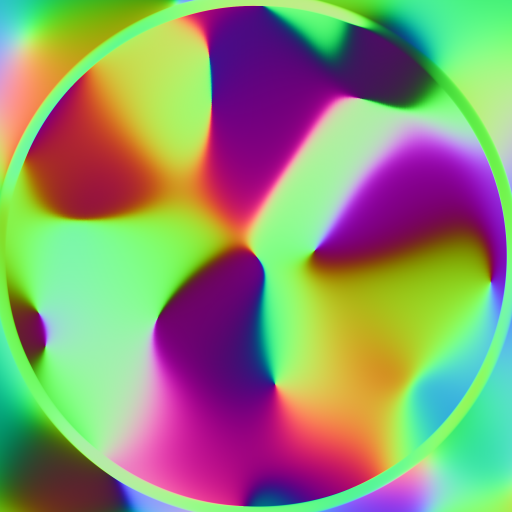
\includegraphics[width=\textwidth]{share/Curl_downscale.png}
\caption{Genomskärning av det slutgiltiga riktningsfället.}
\end{minipage}
\end{figure}

\subsection{Partikelrenderaren} \label{sec:partikelrenderaren}

\begin{figure}[H]
\center
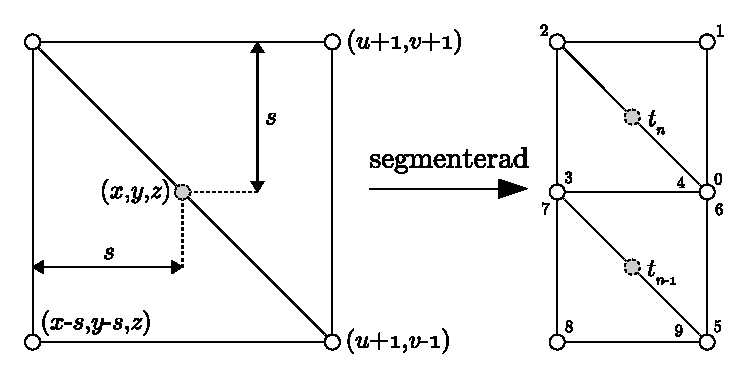
\includegraphics[width=0.5\textwidth]{share/Billboards.eps}
    \caption{(a) en billboard (b) segmenterade billboards.}
\end{figure}

\subsection{Övriga funktioner}

\section{Resultat \& diskussion}

        \subsection{Problem och Lösningar}

        \subsection{Framtida förbättringar}

        \subsection{Projektreflektioner}

    \nocite{*} % Include all.
    \bibliographystyle{abbrv}
    \bibliography{cnpf}
\end{multicols}
\end{document}
